\chapter{Selezione della Modalità di Funzionamento}

%--------------------------------------------------------------------------------------------

Per quanto riguarda la selezione della modalità di funzionamento, è facile intuire che basta
dividere $f_{clk}$ ulteriormente per avere un range di frequenze diverso, come già visto nel
capitolo \ref{segnali_principali}. Aggiungiamo quindi un blocco divisore di frequenza prima
che il segnale arrivi ai contatori e facciamo in modo che la scelta di $f_{out}$ sia
determinata da un comando logico (in questo caso un deviatore).

\begin{figure}[H]
    \centering
    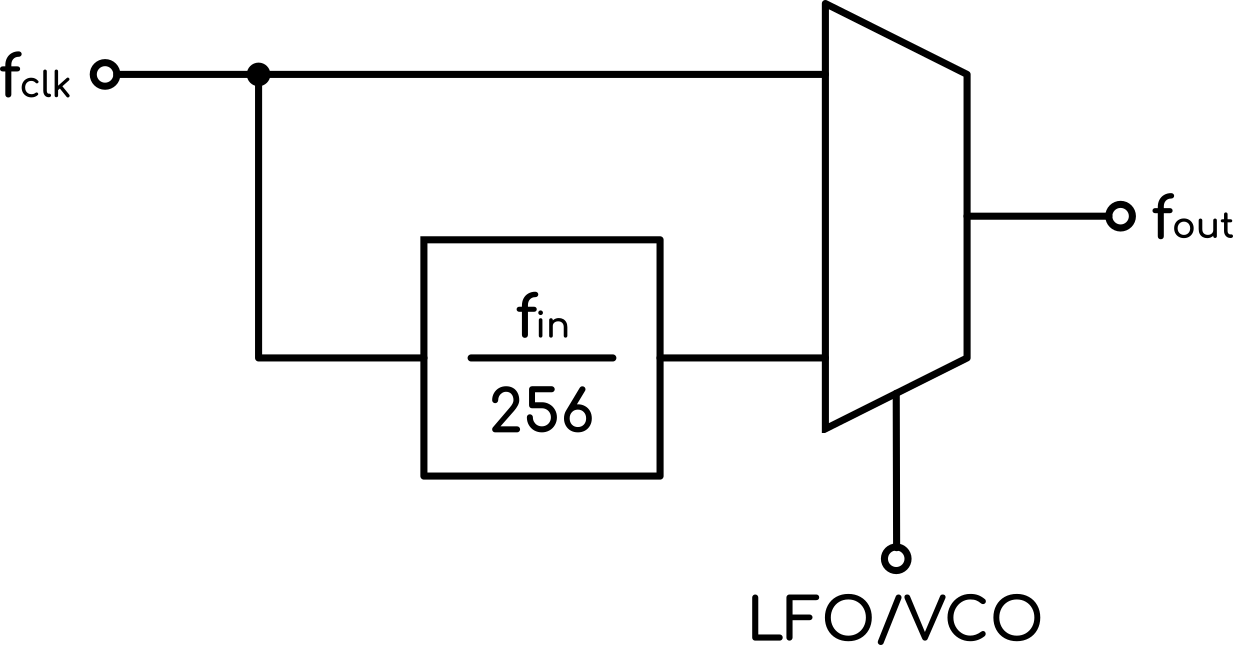
\includegraphics{block_diagrams/mode_selector_block_diagram.png}
    \caption{Schema a blocchi del sottosistema per la selezione della modalità}
    \label{mode_selector_block_diagram}
\end{figure}

Lo schema a blocchi sopra riportato si traduce nel seguente circuito, in cui $f_{clk}$
viene divisa per $256$, traslando il range di funzionamento nell'intervallo
$(\approx0.11\ Hz\div27.5\ Hz)$.

\begin{figure}[H]
    \centering
    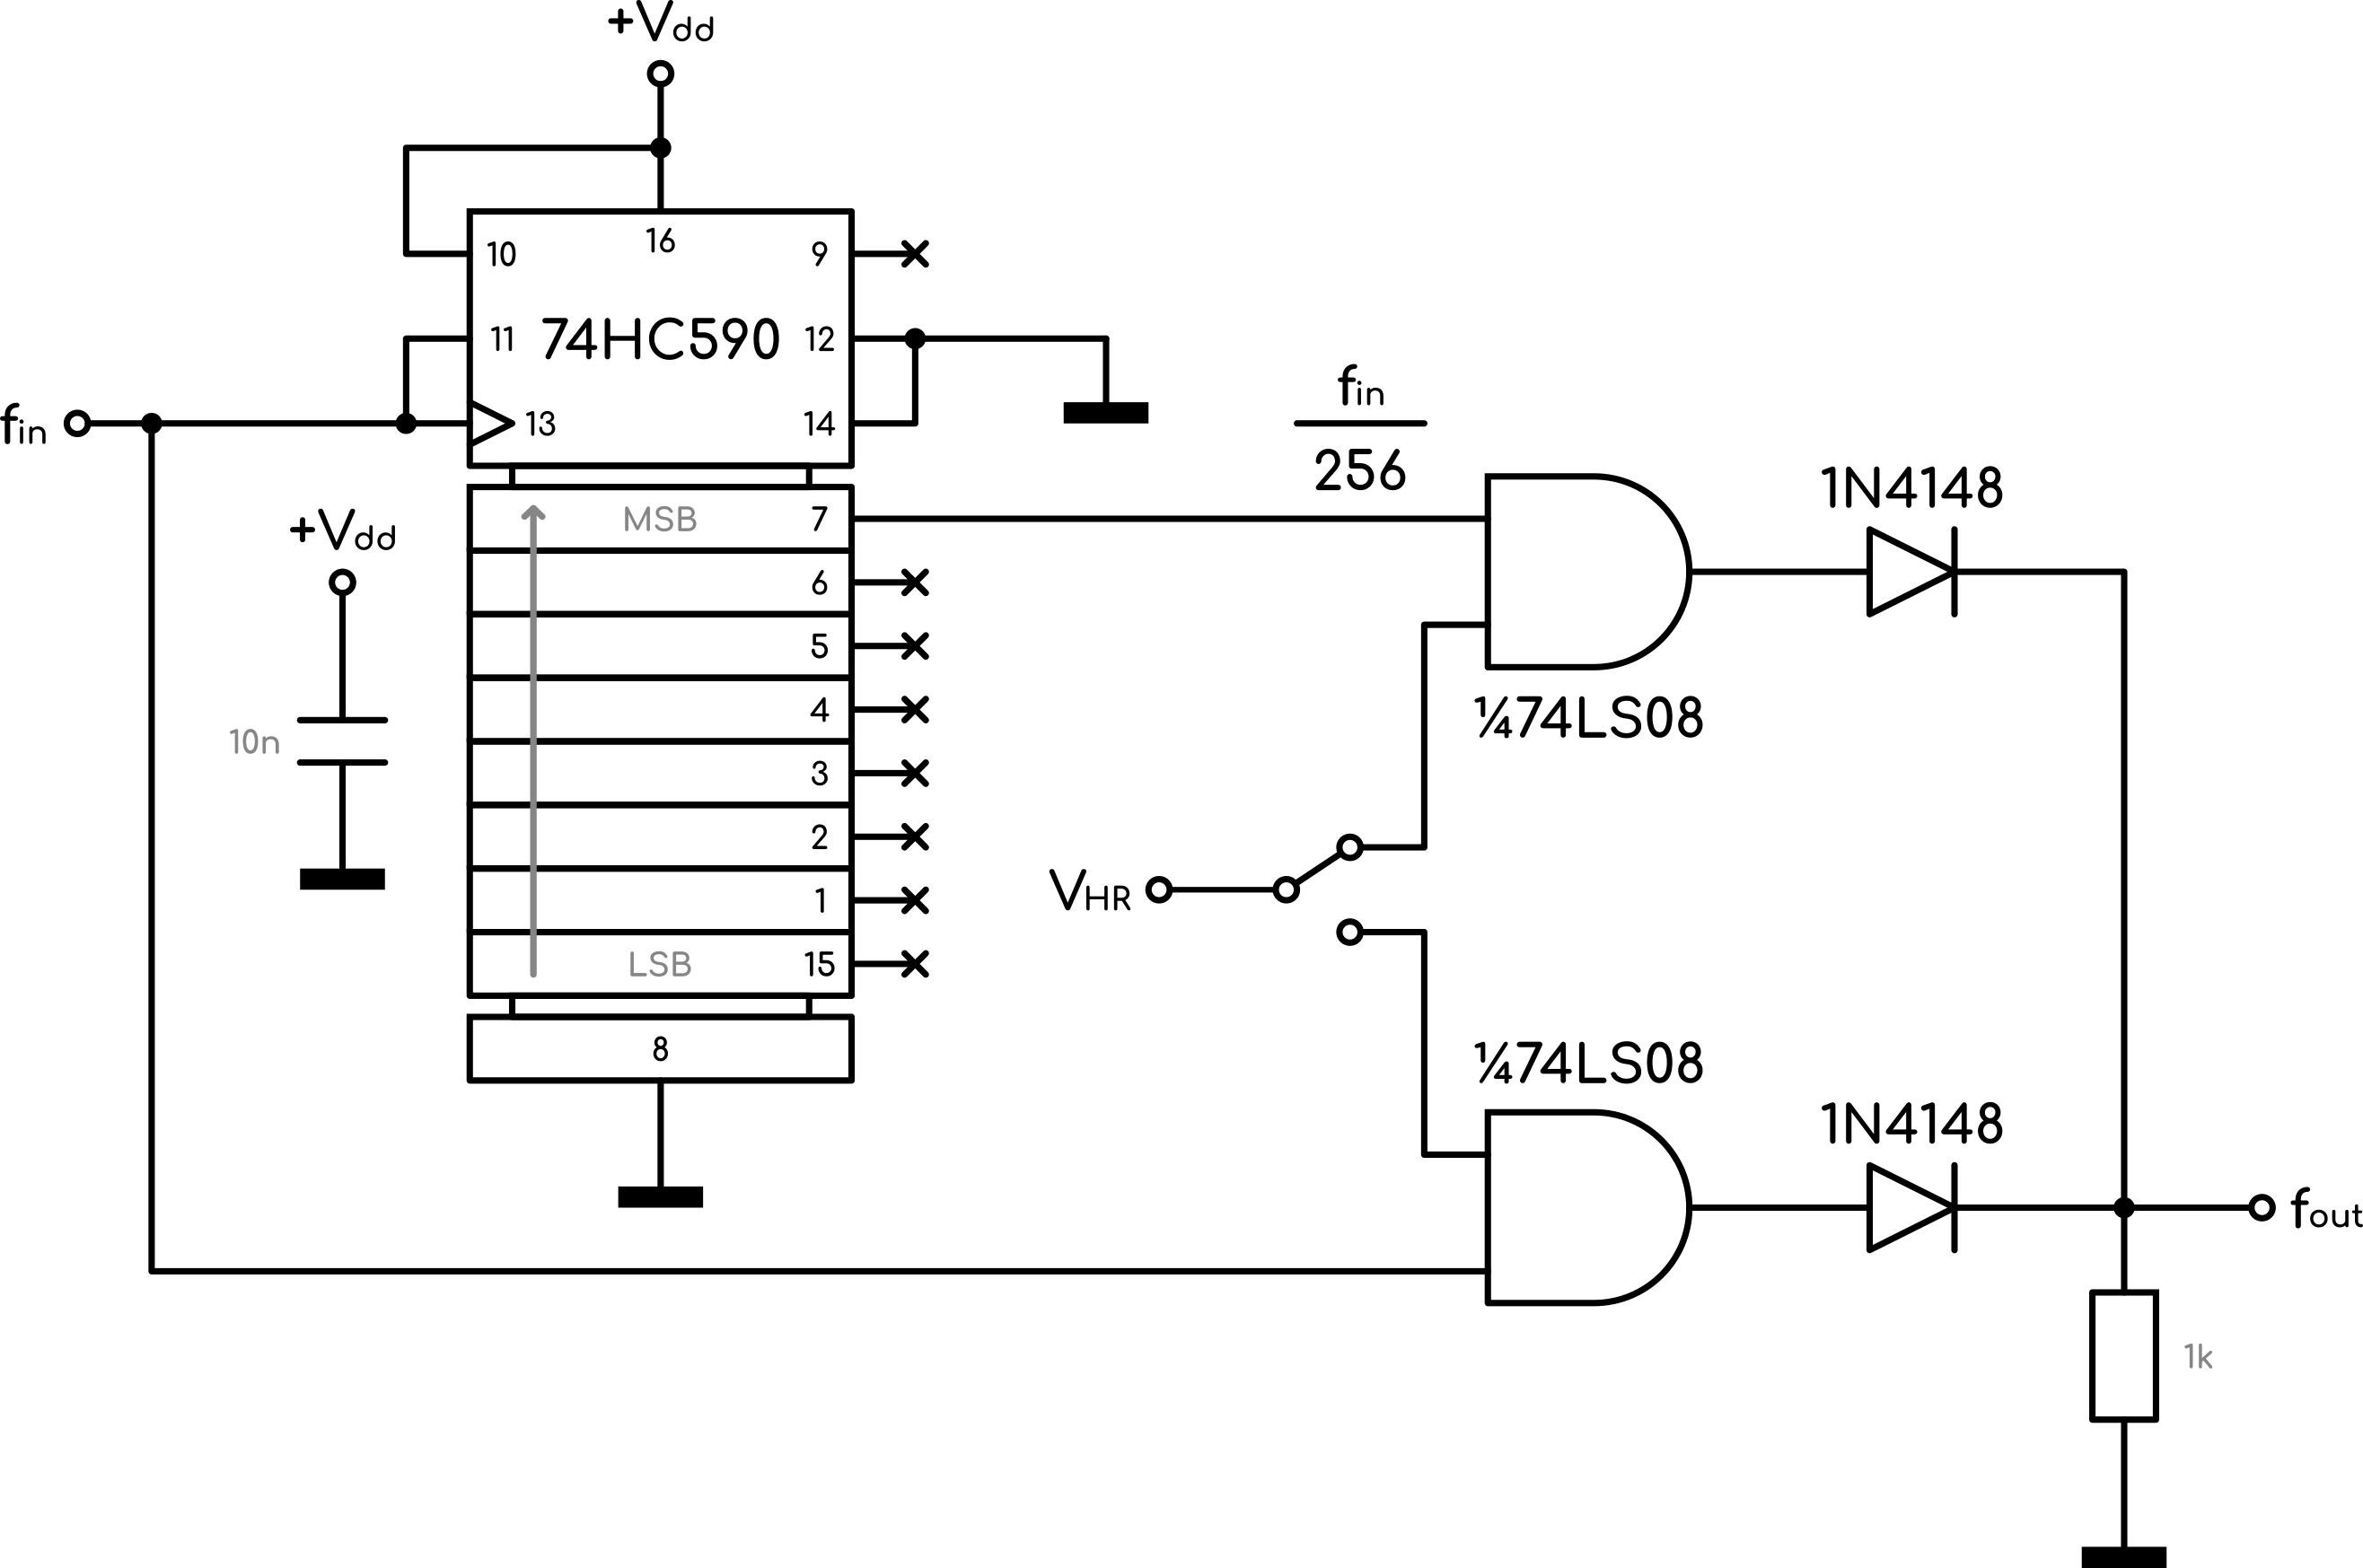
\includegraphics{circuits/mode_selector_circuit.png}
    \caption{Circuito per la selezione della modalità ($+V_{dd}=V_{HR}=+5\ V$)}
    \label{mode_selector_circuit}
\end{figure}

L'unico componente nuovo è un circuito integrato che ospita 4 porte logiche AND, il 74LS08
\cite{74ls08}, utilizzate per il multiplexing del segnale di clock.

Si aggiungono anche dei LED per la visualizzazione dello stato e delle resistenze di pull-down
all'ingresso abilitante delle porte logiche (non rappresentati nello schema in figura
\ref{mode_selector_circuit}).

Possiamo quindi verificare che il circuito divisore di frequenza funzioni correttamente:

\begin{figure}[H]
    \centering

    \begin{subfigure}{.5\textwidth}
        \centering
        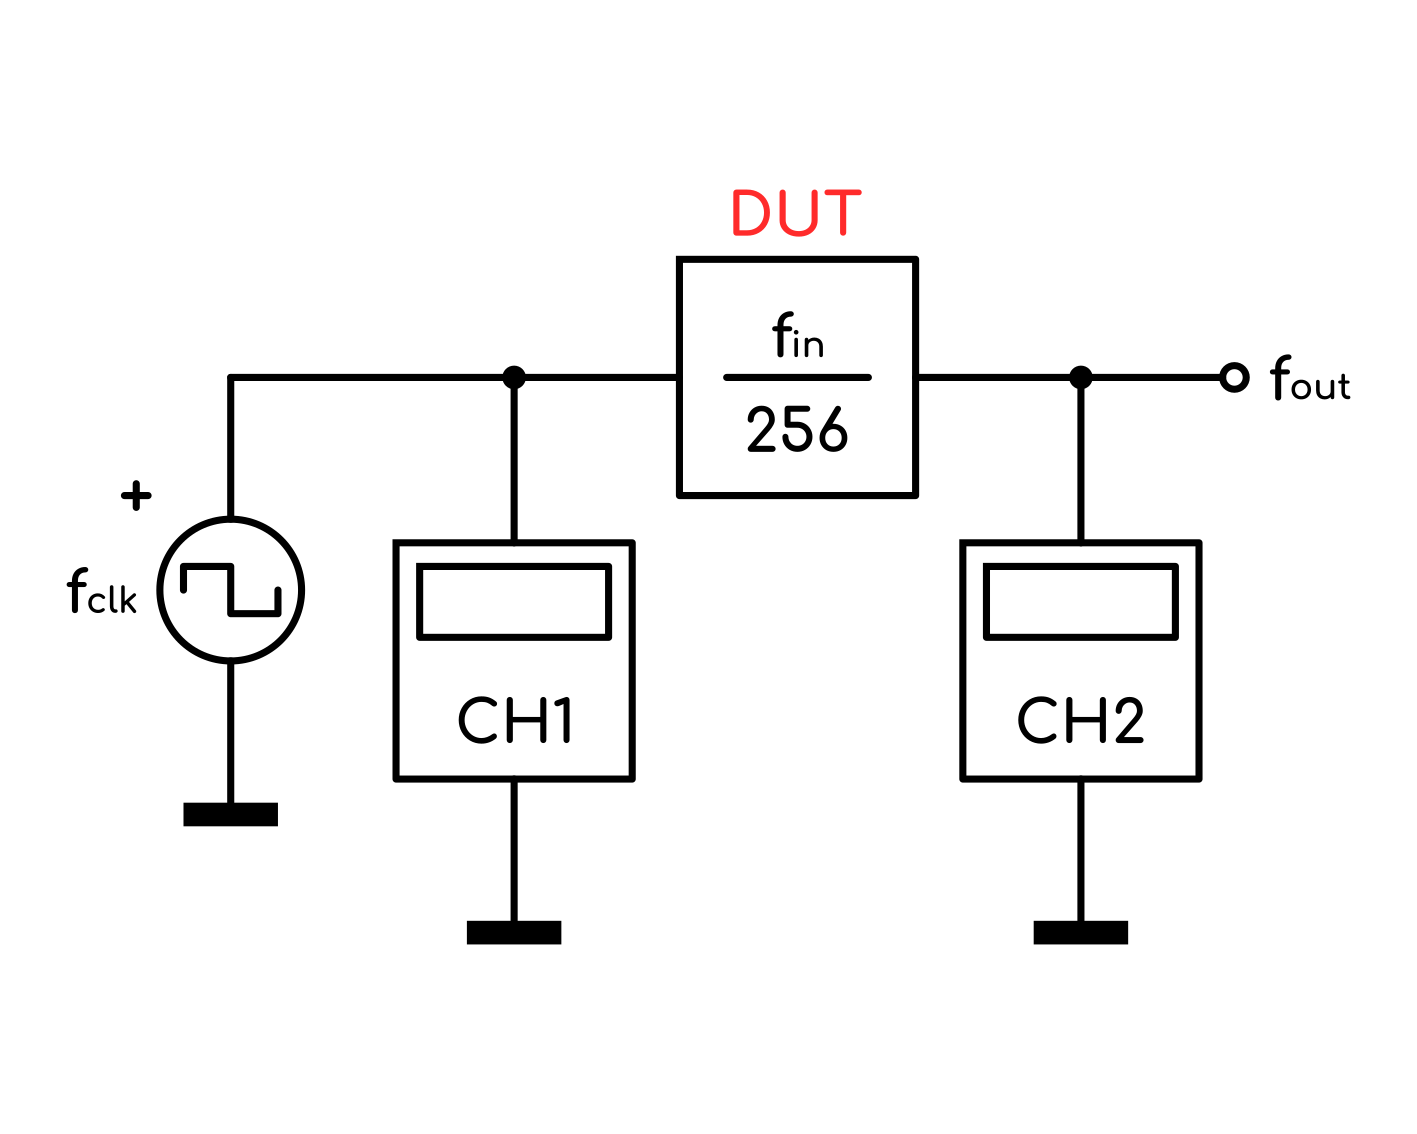
\includegraphics{block_diagrams/mis_LFO_clock_divider.png}
        \caption{Setup di misura}
        \label{mis_LFO_clock_divider}
    \end{subfigure}%
    \begin{subfigure}{.5\textwidth}
        \centering
        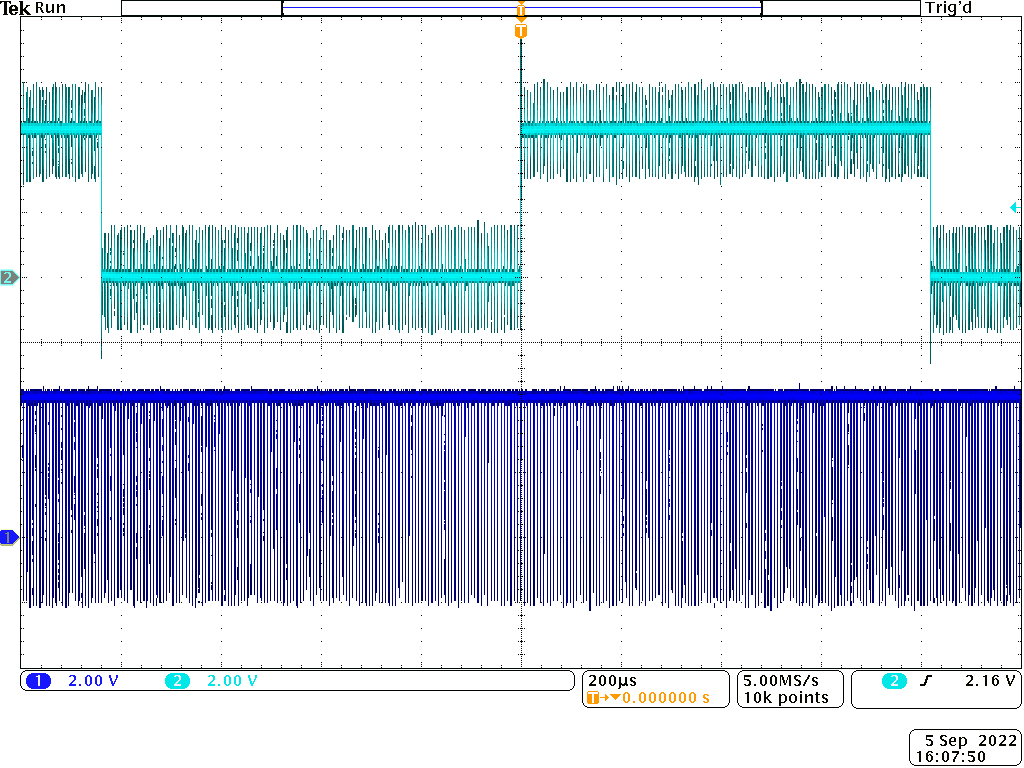
\includegraphics[scale = 0.2]{acquisitions/LFO_divider.png}
        \caption{Acquisizione delle onde ottenute}
        \label{LFO_divider}
    \end{subfigure}

    \caption{Funzionamento del divisore di frequenza}
    \label{freq_divider}
\end{figure}

Spendendo qualche minuto a contare le righe presenti nell'acquisizione (figura \ref{LFO_divider})
si può apprezzare come a 256 cicli di clock del segnale in ingresso ne corrisponda uno
solo in uscita, quindi il circuito funziona come desiderato.

%--------------------------------------------------------------------------------------------
